% !TeX root = ../main.tex
% 原始章节：04-advanced-cpu.Rmd

\chapter{进阶CPU设计实现}\label{chap:04-advanced-cpu}

\section{LainCore简介}\label{sec:04-advanced-cpu-001}

Lain Core 是一款静态双发射的 LoongArch32 Reduced 指令集（以下简称 LA32R）核心，拥有八级的流水线长度，支持两级动态分支预测，具有两路组相连的指令及数据 Cache。

性能方面，核心在 Coremark 仿真中取得 2.7 CM/Mhz 的性能成绩，并在龙芯杯团队赛的十个性能测试点上，取得 0.846 的平均 IPC。 功能方面，核心实现了所有 LA32R 的整数指令及特权指令，支持启动 Linux 操作系统。 核心支持 Verilator 仿真，并可在 FPGA 平台上综合运行。本核心也通过百芯计划完成流片验证，可正常工作。

本项目核心针对 FPGA 进行专门优化，并创新提出基于寄存器重命名的后端前递转发路径优化。Lain Core 在 NSCSCC2023 中，获得了 LA 赛道团队赛第二名，同时也是目前为止龙芯杯历史上运行频率最高的超标量核心。

核心架构如图\ref{fig:04-lain-arch}所示：

\begin{figure}[htbp]
  \centering
  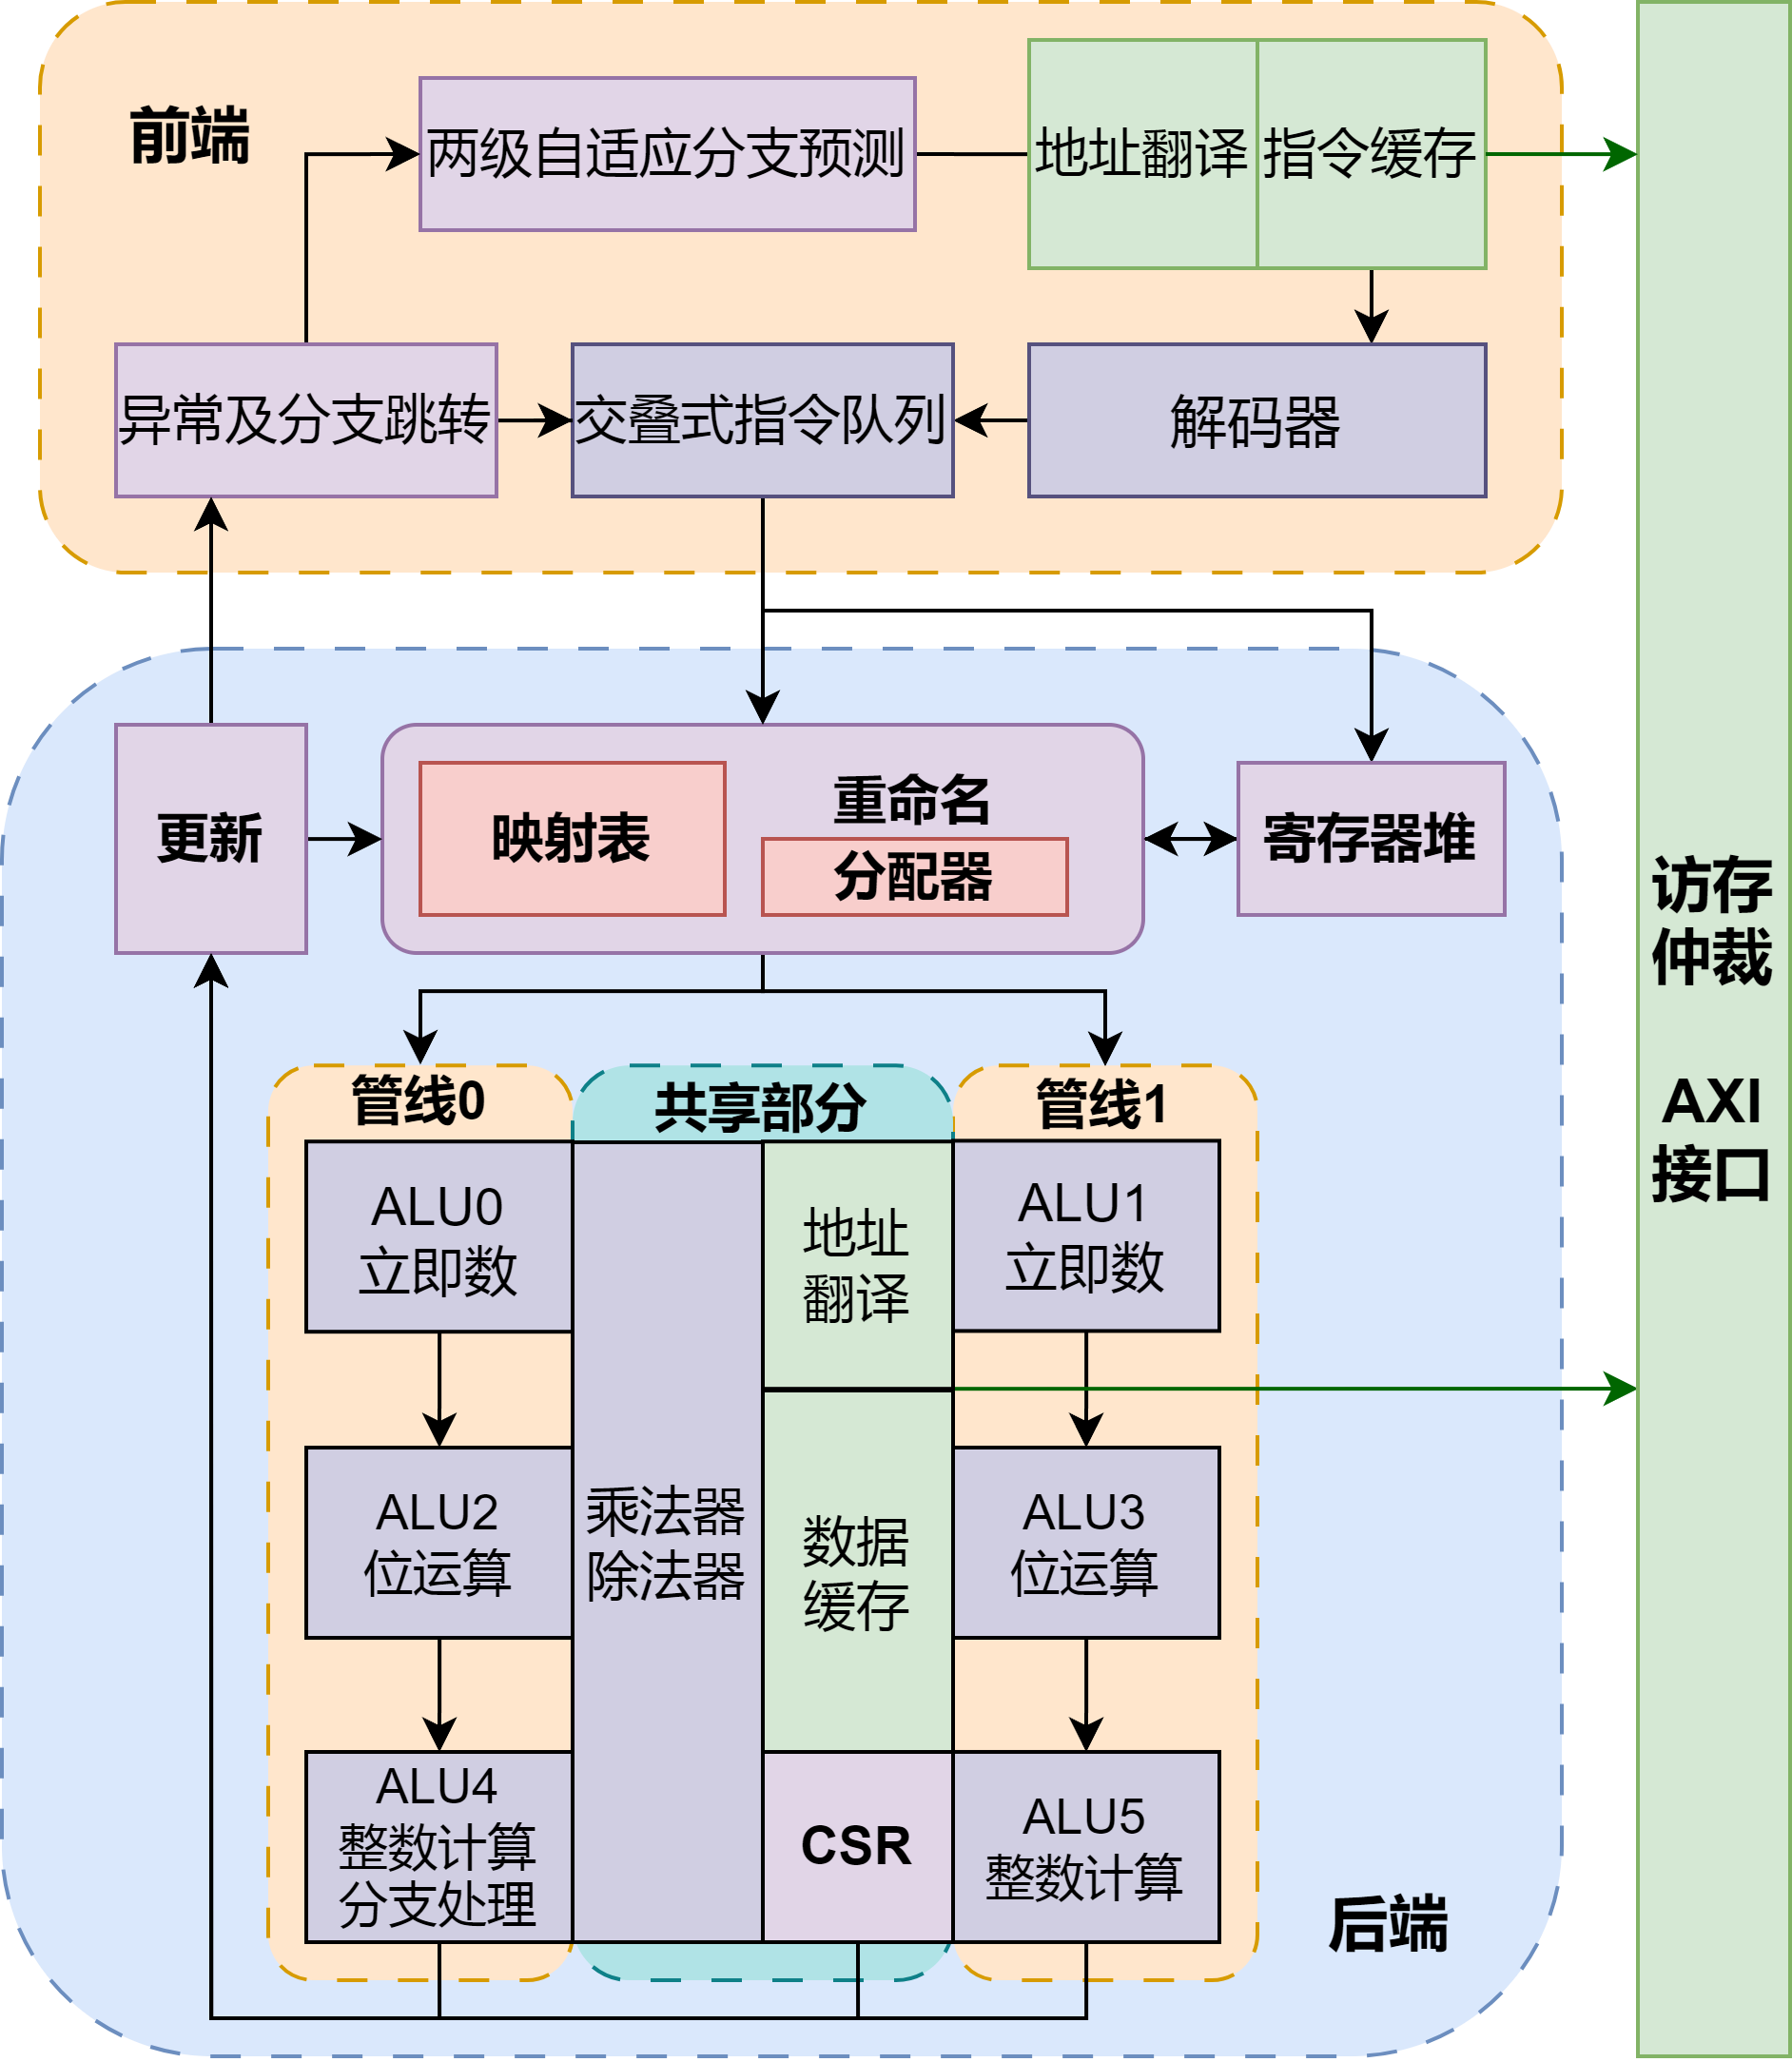
\includegraphics[width=1.0\linewidth]{assets/04/lain-arch.png}
  \caption{LainCore架构图}
  \label{fig:04-lain-arch}
\end{figure}

\section{分支预测}\label{sec:04-advanced-cpu-002}

\begin{itemize}
\tightlist
\item
  代码主要位于\texttt{LainCore/rtl/core\_npc\_complex.sv}文件中
\item
  本小节以LainCore分支预测器为例，介绍如何构建一个简单的二级分支预测器
\item
  本节仅关注如何实现一个简单二级分支预测器，分支预测相关知识参阅教程文档
\end{itemize}

\subsection{整体架构}\label{sec:04-advanced-cpu-003}

\begin{itemize}
\tightlist
\item
  整体上实现了二级分支预测器，架构如图\ref{fig:04-bpu-arch}所示：
\end{itemize}

\begin{figure}[htbp]
  \centering
  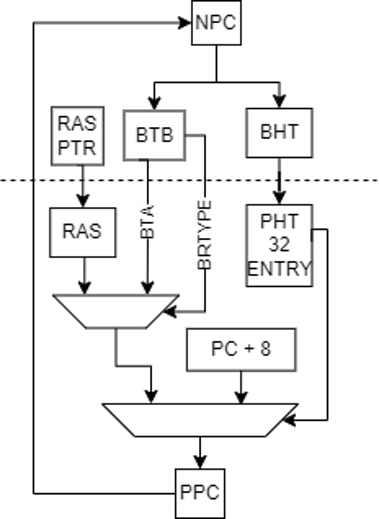
\includegraphics[width=0.5\linewidth]{assets/04/bpu-arch.png}
  \caption{分支预测器架构图}
  \label{fig:04-bpu-arch}
\end{figure}

\begin{itemize}
\tightlist
\item
  由于是顺序双发射架构，预测器每周期给出相邻8对齐两条PC的预测结果
\end{itemize}

\subsection{具体实现}\label{sec:04-advanced-cpu-004}

\begin{itemize}
\item
  \texttt{pipeline.svh}中相关宏定义

  % 代码语言：BookSystemVerilog
\begin{CodeBlock}[language=BookSystemVerilog]
// 定义4种跳转类型
`define _BPU_TARGET_NPC  (2'd0)    // 不跳转
`define _BPU_TARGET_CALL (2'd1)    // 函数调用类型
`define _BPU_TARGET_RETURN (2'd2)  // 调用返回类型
`define _BPU_TARGET_IMM (2'd3)     // 目标地址为pc + imm
\end{CodeBlock}
\item
  \texttt{pipeline.svh}中相关结构体定义

  % 代码语言：BookSystemVerilog
\begin{CodeBlock}[language=BookSystemVerilog]
typedef struct packed {
  logic taken;  // 预测是否跳转
  logic [                31:0] predict_pc ;  // 预测跳转地址
  logic [                 1:0] lphr       ;  // 历史模式信息
  logic [`_BHT_DATA_WIDTH-1:0] history    ;  // 分支历史
  logic [                 1:0] target_type;  // 指令类型
  logic                        dir_type   ;  // 是否条件跳转
  logic [`_RAS_ADDR_WIDTH-1:0] ras_ptr;  // RAS栈指针
} bpu_predict_t;  // 分支预测信息

typedef struct packed {
  logic                        miss       ;  // 预测失败
  logic [                31:0] pc         ;  // 预测失败的PC
  logic                        true_taken ;  // 是否跳转
  logic [                31:0] true_target;  // 跳转目标
  logic [                 1:0] lphr       ;  // 预测信息携带的旧的lphr，更新时需要进一步计算
  logic [`_BHT_DATA_WIDTH-1:0] history    ;  // 预测信息携带的旧的历史，更新时需要进一步计算

  logic need_update         ;  // BPU是否需要更新
  logic true_conditional_jmp;  // 是否是条件跳转

  logic ras_miss_type;  // 是否需要更新RAS

  logic[1:0] true_target_type;  // 指令分支类型

  logic [`_RAS_ADDR_WIDTH-1:0] ras_ptr;  // 预测信息携带的旧的RAS栈指针
} bpu_correct_t;  // 正确的分支信息，也是BPU更新信息


\end{CodeBlock}
\item
  顶层接口定义：

  % 代码语言：BookSystemVerilog
\begin{CodeBlock}[language=BookSystemVerilog]
module core_npc (
  input  logic              clk       ,
  input  logic              rst_n     ,
  input  logic              rst_jmp   ,  // 流水线冲刷信号
  input  logic [31:0]       rst_target,  // 流水线冲刷时的目标地址
  input  logic              f_stall_i ,  // 暂停信号
  output logic [31:0]       pc_o      ,
  output logic [31:0]       npc_o     ,
  output logic [ 1:0]       valid_o   ,  // 2'b00 | 2'b01 | 2'b11 | 2'b10
  output bpu_predict_t [1:0]predict_o ,
  input  bpu_correct_t      correct_i
);
\end{CodeBlock}
\item
  本节一些通用的命名含义：
\end{itemize}

\begin{longtable}[]{@{}lll@{}}
\toprule\noalign{}
名称 & 全称 & 含义 \\
\midrule\noalign{}
\endhead
\bottomrule\noalign{}
\endlastfoot
pc & program counter & 程序计数器 \\
npc & next pc & 下一周期的pc \\
ppc & predicted pc & pc的预测结果 \\
\_q & & 触发器输出端的标识 \\
lphr & local pattern history reg & 部模式历史寄存器 \\
\end{longtable}

\subsubsection{RAS实现}\label{sec:04-advanced-cpu-005}

\begin{itemize}
\item
  RAS（Return Address Stack）相关知识见教程文档
\item
  一般的RAS的大小不超过16，\textbf{LainCore中RAS大小为8}
\item
  定义存储结构\texttt{logic{[}7:0{]}{[}31:0{]}\ ras\_q;}
\item
  定义读写指针\texttt{logic{[}2:0{]}\ ras\_w\_ptr\_q,\ ras\_ptr\_q;}
\item
  定义分支预测逻辑中用到的RAS值的寄存器\texttt{logic{[}31:0{]}\ ppc\_ras\_q;}
\item
  RAS写入：在预测指令为CALL类型指令时被写入

  % 代码语言：BookSystemVerilog
\begin{CodeBlock}[language=BookSystemVerilog]
// 如果pc是CALL类型指令且流水线不发生暂停
if(pc_is_call && !f_stall_i) begin
  // 按照指令是第一条还是第二条计算写入的PC值，并进行写入
  ras_q[ras_w_ptr_q] <= {pc[31:3], 3'b000} + (inst_0_jmp ? 32'd4 : 32'd8);
  // 更新写指针
  ras_w_ptr_q <= ras_w_ptr_q + 3'd1;
  // 更新读指针
  ras_ptr_q <= ras_ptr_q + 3'd1;
end
\end{CodeBlock}
\item
  RAS读出：在预测指令为RETURN类型指令时读出

  % 代码语言：BookSystemVerilog
\begin{CodeBlock}[language=BookSystemVerilog]
// 在第一个周期将栈顶元素读出到寄存器，优化时序
always_ff @(posedge clk) begin
	ppc_ras_q <= {ras_q[ras_ptr_q][31:2], 2'b00};
end

// 第二周期，如果pc是RETURN类型指令且流水线不发生暂停
if(pc_is_return && !f_stall_i) begin
	// 更新读写指针
	ras_w_ptr_q <= ras_w_ptr_q - 3'd1;
	ras_ptr_q <= ras_ptr_q - 3'd1;
end
\end{CodeBlock}
\item
  RAS更新：在分支预测失败时更新

  % 代码语言：BookSystemVerilog
\begin{CodeBlock}[language=BookSystemVerilog]
// RETURN MISS: 更新读写指针
// CALL   MISS: 更新读写指针和RAS栈顶元素
if(correct_i.miss || correct_i.ras_miss_type) begin
  // 更新写指针
  ras_w_ptr_q <= correct_i.ras_ptr + 3'd1;
  // 更新读指针
  ras_ptr_q <= correct_i.ras_ptr;
  // CALL 类型的MISS 还需要更新RAS栈顶元素
  if(correct_i.true_target_type == `_BPU_TARGET_CALL) begin
    ras_q[correct_i.ras_ptr] <= correct_i.pc + 3'd4;
  end
end
\end{CodeBlock}
\end{itemize}

\subsubsection{BTB实现}\label{sec:04-advanced-cpu-006}

\begin{itemize}
\item
  BTB（Branch Target Buffer）相关知识见教程文档
\item
  BTB被分为两个部分：地址部分（btb部分）和信息部分（info部分）
\item
  \textbf{注意：}历史遗留问题，代码命名中btb仅指代地址缓存，info指代指令信息缓存，\textbf{切勿将代码btb与教程中BTB含义混淆}
\item
  btb部分包含1024个表项，分2个BANK，结构为2 * 512 entry
\item
  info部分包含512个表项，分2个BANK，结构为2 * 256 entry
\item
  定义btb ram相关变量：

  % 代码语言：BookSystemVerilog
\begin{CodeBlock}[language=BookSystemVerilog]
logic[8:0] btb_waddr,btb_raddr;
logic[1:0] btb_we;
logic[31:0] btb_wdata;
logic[1:0][31:0] btb_rdata;
\end{CodeBlock}
\item
  定义info ram相关变量：

  % 代码语言：BookSystemVerilog
\begin{CodeBlock}[language=BookSystemVerilog]
typedef struct packed {
  logic [1:0] target_type; // 0 npc, 1 call, 2 return, 3 imm
  logic conditional_jmp;   // 0：非条件跳转；1：条件跳转
  logic [4:0] history;     // 分支历史
  logic [5:0] tag;         // pc对应的tag，确定pc身份
} branch_info_t;

logic[7:0] info_waddr,info_raddr;
logic[1:0] info_we;
branch_info_t winfo;
branch_info_t [1:0]rinfo_q;
\end{CodeBlock}
\item
  存储结构定义：

  % 代码语言：BookSystemVerilog
\begin{CodeBlock}[language=BookSystemVerilog]
// 创建两个 btb 和 info mem，用于写更新时区别开来。
for(genvar p = 0 ; p < 2 ; p++) begin  
  simpleDualPortRamRE #(
    .dataWidth(30 ),
    .ramSize  (512),
    .latency  (1  ),
    .readMuler(1  )
  ) btb_table (
    .clk     (clk       ),
    .rst_n   (rst_n     ),
    .addressA(btb_waddr ),
    .we      (btb_we[p] ),
    .addressB(btb_raddr ),
    .re      (!f_stall_i),
    .inData  (btb_wdata[31:2]),
    .outData (btb_rdata[p][31:2])
  );
  assign btb_rdata[p][1:0] = '0;
  simpleDualPortLutRam #(
    .dataWidth($bits(branch_info_t)),
    .ramSize  (256),
    .latency  (1  ),
    .readMuler(1  )
  ) info_table (
    .clk     (clk       ),
    .rst_n   (rst_n     ),
    .addressA(info_waddr),
    .we      (info_we[p] | !rst_n_q),
    .addressB(info_raddr ^ rst_addr_q),
    .re      (!f_stall_i),
    .inData  (winfo),
    .outData (rinfo_q[p])
  );
end
\end{CodeBlock}
\item
  btb读写逻辑：

  % 代码语言：BookSystemVerilog
\begin{CodeBlock}[language=BookSystemVerilog]
assign btb_raddr = npc[11:3];              // 读地址来自NPC
assign btb_waddr = correct_i.pc[11:3];     // 写地址来自BPU更新请求
assign btb_wdata = correct_i.true_target;  // 将正确的跳转目标写入btb ram
always_comb begin
  btb_we = '0;  // 默认不发生写入
  // 仅更新PC对应的BANK
  // 仅CALL和IMM类型指令需要缓存目标地址
  // 因为：NPC类型不跳转，RETURN类型地址来自RAS
  btb_we[correct_i.pc[2]] = correct_i.need_update && 
                           (correct_i.true_target_type == `_BPU_TARGET_CALL ||
                            correct_i.true_target_type == `_BPU_TARGET_IMM);
end
\end{CodeBlock}
\item
  info读写逻辑

  % 代码语言：BookSystemVerilog
\begin{CodeBlock}[language=BookSystemVerilog]
assign info_raddr = npc[10:3];          // 读地址来自NPC
assign info_waddr = correct_i.pc[10:3]; // 写地址来自BPU更新请求
always_comb begin
	info_we = '0;  // 默认不发生写入
  // 仅更新PC对应的BANK
	info_we[correct_i.pc[2]] = correct_i.need_update;
end
always_comb begin
  // 复位时写入信息应采用NPC类型
	winfo.target_type = rst_n_q ? correct_i.true_target_type : `_BPU_TARGET_NPC;
	// 更新条件跳转信息
  winfo.conditional_jmp = correct_i.true_conditional_jmp;
	// 滚动更新分支历史
  winfo.history = {correct_i.history[3:0], correct_i.true_taken};
	// 更新PC对应的tag
  winfo.tag = get_tag(correct_i.pc);
end
\end{CodeBlock}
\end{itemize}

\subsubsection{PHT实现}\label{sec:04-advanced-cpu-007}

\begin{itemize}
\item
  PHT（Pattern History Table）相关知识见教程文档
\item
  本文BPU架构中，PHT共32个表项
\item
  定义PHT相关信号：

  % 代码语言：BookSystemVerilog
\begin{CodeBlock}[language=BookSystemVerilog]
logic level2_we;
logic [4:0] level2_waddr;
logic [1:0] level2_wdata;
logic [1:0][4:0] level2_raddr;
logic [1:0][1:0] level2_cnt;  // PHT的读出数据
\end{CodeBlock}
\item
  存储结构定义：

  % 代码语言：BookSystemVerilog
\begin{CodeBlock}[language=BookSystemVerilog]
for(genvar p = 0 ; p < 2; p++) begin
  simpleDualPortLutRam #(
    .dataWidth(2 ),
    .ramSize  (32),
    .latency  (0 ),  // 注意这里的延迟是0，
    .readMuler(1 )
  ) l2_table (
    .clk     (clk            ),
    .rst_n   (rst_n          ),
    .addressA(level2_waddr   ),
    .we      (level2_we      ),
    .addressB(level2_raddr[p]),
    .re      (1'b1           ),
    .inData  (level2_wdata   ),
    .outData (level2_cnt[p]  )
  );
end
\end{CodeBlock}
\item
  读写逻辑：

  % 代码语言：BookSystemVerilog
\begin{CodeBlock}[language=BookSystemVerilog]
// 按照两位饱和计数器的规范计算要写入的pht表项信息
assign level2_wdata = gen_next_lphr(correct_i.lphr, correct_i.true_taken);
// 写入地址是更新信息中携带的分支历史
assign level2_waddr = correct_i.history;
// 是条件跳转的指令才会更新这个表
assign level2_we = correct_i.true_conditional_jmp && correct_i.need_update;
for(genvar p = 0 ; p < 2; p++) begin
  // 使用分支历史来寻址pht
  assign level2_raddr[p] = rinfo_q[p].history;
end
\end{CodeBlock}
\end{itemize}

\subsubsection{分支预测}\label{sec:04-advanced-cpu-008}

\begin{itemize}
\item
  本阶段主要任务如下：

  \begin{itemize}
  \tightlist
  \item
    跳转方向预测
  \item
    有效性标记（标记输出的PC的有效性）
  \item
    跳转目标预测
  \item
    生成分支预测信息
  \end{itemize}
\item
  跳转方向预测：

  % 代码语言：BookSystemVerilog
\begin{CodeBlock}[language=BookSystemVerilog]
// 定义相关信号
logic [1:0] branch_need_jmp;  // 是否需要跳转
logic [1:0] tag_match;  // PC与读出的TAG是否匹配

// 预测逻辑，valid_q参看指令有效性标记
for(genvar p = 0 ; p < 2; p++) begin
  always_comb begin
    branch_need_jmp[p] = '0; // 默认不跳转
    // 判断info表项是否被PC命中
    assign tag_match[p] = rinfo_q[p].tag == get_tag(pc);
    // 如果PC命中info表项且是分支指令
    if(rinfo_q[p].target_type != `_BPU_TARGET_NPC && tag_match[p]) begin
      // 以下条件判断PC是否对应无条件跳转指令
      if(rinfo_q[p].target_type != `_BPU_TARGET_IMM || !rinfo_q[p].conditional_jmp) begin
        branch_need_jmp[p] = /*'1*/valid_q[p];
      end
      else begin
        // PC被判定为条件跳转指令
        // 根据PHT的结果判断是否跳转
        branch_need_jmp[p] = level2_cnt[p][1] && valid_q[p];
      end
    end
  end
end
\end{CodeBlock}
\item
  指令有效性标记

  \begin{itemize}
  \tightlist
  \item
    在完成指令跳转情况判断后就可以对npc的有效性进行标记
  \item
    分两个周期进行

    \begin{itemize}
    \tightlist
    \item
      第一周期：根据npc判断第一条指令是否有效
    \item
      第二周期：根据预测跳转信息判断第二条指令是否有效
    \end{itemize}
  \end{itemize}

  % 代码语言：BookSystemVerilog
\begin{CodeBlock}[language=BookSystemVerilog]
// 定义相关信号
// output logic [1:0] valid_o; 标记BPU输出PC的有效性
logic[1:0] valid_q;  // nvalid缓存一拍，与npc流动一致
logic[1:0] nvalid;   // 表示由npc值决定的有效性

// nvalid 逻辑
always_comb begin
  // 默认两条指令都有效
  nvalid = 2'b11;
  // 当npc的其实位置是相邻至指令的第二条指令
  // 将第一条指令无效化
  if(npc[2]) begin
    nvalid[0] = '0;
  end
end

// valid_o 逻辑
always_comb begin
  valid_o = valid_q & {!f_stall_i, !f_stall_i};
  // 若第一条指令预测跳转，将第二条指令无效化
  if(inst_0_jmp) begin
    valid_o[1] = '0;
  end
end

// 更新valid_q
always_ff @(posedge clk) begin
  if(!rst_n) begin
    valid_q <= 2'b11;
  end
  else begin
    // 当流水线不暂停或冲刷流水线时写入
    if(!f_stall_i || rst_jmp) begin
      valid_q <= nvalid;
    end
  end
end
\end{CodeBlock}
\item
  跳转目标预测

  \begin{itemize}
  \tightlist
  \item
    目标地址共有4个来源

    \begin{itemize}
    \tightlist
    \item
      PPC\_RAS\_Q: RAS 方式预测的下一个跳转地址
    \item
      PPC\_BTB: BTB 方式预测的下一个跳转地址
    \item
      PPC\_PLUS8: 不预测跳转情况下，正常 +8
    \item
      JPC: 后端刷新管线的跳转地址
    \end{itemize}
  \end{itemize}

  % 代码语言：BookSystemVerilog
\begin{CodeBlock}[language=BookSystemVerilog]
always_comb begin
  // npc 默认为 align(pc, 8) + 8
  npc = ppc_plus8;
  if(branch_need_jmp[0]) begin
    // 如果第一条指令预测跳转，根据类型选择目标地址
    npc = rinfo_q[0].target_type == `_BPU_TARGET_RETURN ? ppc_ras_q : raw_ppc_btb[0];
  end else if(branch_need_jmp[1]) begin
    // 如果第一条指令跳转，自然无需再判断第二条指令的目标地址
    // 如果第二条指令预测跳转，根据类型选择目标地址
    npc = rinfo_q[1].target_type == `_BPU_TARGET_RETURN ? ppc_ras_q : raw_ppc_btb[1];
  end
  // 冲刷流水线优先级最高
  if(rst_jmp) begin
    npc = jpc;
  end
end
\end{CodeBlock}
\item
  分支信息输出

  % 代码语言：BookSystemVerilog
\begin{CodeBlock}[language=BookSystemVerilog]
always_comb begin
  if(branch_need_jmp[0]) begin
    predict_o[0].taken = '1;
  end
  else if(branch_need_jmp[1]) begin
    predict_o[1].taken = '1;
  end
end

always_comb begin
  predict_o[0].predict_pc = npc;
  predict_o[1].predict_pc = npc;
  predict_o[0].lphr = level2_cnt[0];
  predict_o[1].lphr = level2_cnt[1];
  predict_o[0].history = rinfo_q[0].history;
  predict_o[1].history = rinfo_q[1].history;
  predict_o[0].target_type = rinfo_q[0].target_type;
  predict_o[1].target_type = rinfo_q[1].target_type;
  predict_o[0].dir_type = rinfo_q[0].conditional_jmp;
  predict_o[1].dir_type = rinfo_q[1].conditional_jmp;
  predict_o[0].ras_ptr = ras_ptr_q;
  predict_o[1].ras_ptr = ras_ptr_q;
end
\end{CodeBlock}
\end{itemize}

\section{指令译码}\label{sec:04-advanced-cpu-009}

\begin{itemize}
\item
  手动构建译码器比较简单，一般采用AND-OR结构
\item
  可参考\url{https://gitee.com/loongson-edu/open-la500/blob/master/id_stage.v}
\item
  本节介绍如何使用 LainCore 提供的解码器脚本生成解码器，可大大提升开发效率
\end{itemize}

\subsection{配置脚本运行环境}\label{sec:04-advanced-cpu-010}

\subsubsection{安装Java}\label{sec:04-advanced-cpu-011}

\begin{itemize}
\item
  运行如下命令

  % 代码语言：BookShell
\begin{CodeBlock}[language=BookShell]
apt install openjdk-21-jre-headless  # 安装Java运行环境
apt install openjdk-21-jdk-headless  # 安装Java开发环境
\end{CodeBlock}
\item
  测试Java运行环境

  % 代码语言：BookShell
\begin{CodeBlock}[language=BookShell]
$ java --version
openjdk 21.0.3 2024-04-16
OpenJDK Runtime Environment (build 21.0.3+9-Ubuntu-1ubuntu122.04.1)
OpenJDK 64-Bit Server VM (build 21.0.3+9-Ubuntu-1ubuntu122.04.1, mixed mode, sharing)
\end{CodeBlock}
\item
  测试Java开发环境

  % 代码语言：BookShell
\begin{CodeBlock}[language=BookShell]
$ javac --version
javac 21.0.3
\end{CodeBlock}
\end{itemize}

\subsubsection{安装Scala}\label{sec:04-advanced-cpu-012}

\begin{itemize}
\item
  下载安装包

  % 代码语言：BookShell
\begin{CodeBlock}[language=BookShell]
wget https://downloads.lightbend.com/scala/2.11.12/scala-2.11.12.deb
\end{CodeBlock}
\item
  安装

  % 代码语言：BookShell
\begin{CodeBlock}[language=BookShell]
sudo dpkg -i scala-2.11.12.deb
\end{CodeBlock}
\item
  检查

  % 代码语言：BookShell
\begin{CodeBlock}[language=BookShell]
$ scala -version
Scala code runner version 2.11.12 -- Copyright 2002-2017, LAMP/EPFL
\end{CodeBlock}
\end{itemize}

\subsubsection{安装sbt}\label{sec:04-advanced-cpu-013}

\begin{itemize}
\tightlist
\item
  \textbf{该步骤需要正确配置代理}
\end{itemize}

% 代码语言：BookShell
\begin{CodeBlock}[language=BookShell]
echo "deb https://repo.scala-sbt.org/scalasbt/debian all main" | sudo tee /etc/apt/sources.list.d/sbt.list
echo "deb https://repo.scala-sbt.org/scalasbt/debian /" | sudo tee /etc/apt/sources.list.d/sbt_old.list
curl -sL "https://keyserver.ubuntu.com/pks/lookup?op=get&search=0x2EE0EA64E40A89B84B2DF73499E82A75642AC823" | sudo apt-key add
sudo apt-get update
sudo apt-get install sbt
\end{CodeBlock}

\subsection{脚本使用}\label{sec:04-advanced-cpu-014}

\subsubsection{编写解码器相关信息}\label{sec:04-advanced-cpu-015}

\begin{itemize}
\item
  代码位于\texttt{LainCore/src/simple-decoder}文件夹下
\item
  脚本通过编写JSON文件定义解码器

  \begin{itemize}
  \item
    脚本支持读入多个JSON文件
  \item
    脚本一次性读入所有JSON后才进行分析，在A脚本中定义的内容可在B脚本中使用
  \item
    JSON文件规范如下：

    % 代码语言：BookJSON
\begin{CodeBlock}[language=BookJSON]
{
  // 支持3种指令信号值的定义方式
  "signal_values": {
    // 列表形式
    // 最终会在decoder.svh中生成对应宏定义
    "signal_name0": [
      "S0_VALUE0",  // 0
      "S0_VALUE1",  // 1
      "s0_VALUE3"   // 2
    ],

		// MAP形式
    // 最终会在decoder.svh中生成对应宏定义
    // 宏定义值与此处赋值相同
    "signal_name1": {
      "S1_VALUE0" : 0,
      "S1_VALUE1" : 0,
      "S1_VALUE2" : 1,
      "S1_VALUE3" : 2,
      "S1_VALUE4" : 3,
      "S1_VALUE5" : 4
    },

    // 真值形式
    // 不会生成宏定义
    "signal_name2": [false, true]
  },
  "signals": {
    // 信号定义包括三个键值对
    // length：信号位宽
    // stage：信号最后一个有效的流水级，此后信号被抛弃，用于生成信号在流水线中传递的接线函数
    // default：信号默认值，需保证与信号位宽一致
    "signal_name0": {
      "length": 2,
      "stage": "ex",
      "default": "S0_VALUE0"
    },
    "signal_name1": {
      "length": 3,
      "stage": "m1",
      "default": "S1_VALUE0"
    },
    "signal_name2": {
      "length": 1,
      "stage": "m2",
      "default": false
    }

  },
  "instructs": {
    // 指令解码信息定义
    // opcode：指令标识码，原则上支持掩码形式，即支持形如“01010101----0101”的形式
    // signal_namex：指令关注的信号，例如addi指令需要将alu_op信号设置为"ADD"
    // 指令仅需要设置自己会影响到的信号，其余信号会采用默认值
    "instruct_name0": {
      "opcode": "01010101",
      "signal_name0": "S0_VALUE0",
      "signal_name1": "S1_VALUE0",
      "signal_name2": false
    },
    "instruct_name1": {
      "opcode": "01010110",
      "signal_name0": "S0_VALUE1",
      "signal_name2": true
    },
    "instruct_name2": {
      "opcode": "01010110"
    }
  }
}
\end{CodeBlock}
  \end{itemize}
\item
  脚本Config文件

  % 代码语言：BookScala
\begin{CodeBlock}[language=BookScala]
object Config {
  val useJson = true  // 也可以直接编写SpinalHDL格式的解码文件，此时设置该值为false，但是此功能还不完整
  // 定义CPU流水级，需要考虑顺序，需与JSON中出现的一致
  val stages: List[String] = List("is", "ex", "m1", "m2", "wb")
  // 如果有想要添加到decoder.svh的其他和解码无关常量
  val constPatch: String =
    """
      ...
      |""".stripMargin

  val debug = true  // 控制添加指令原本信息
  val checkInvalidInst = true  // 检查无效指令
  val exceptionStage = "m1"  // 例外处理在哪一级？
  val bitWidth = 32  // 位宽
  val targetDirectory = "rtl"  // 脚本输出路径
  val defaultInstSet: InstSet = LoongArch32  // 无需修改
}
\end{CodeBlock}
\end{itemize}

\subsubsection{运行脚本}\label{sec:04-advanced-cpu-016}

\begin{itemize}
\item
  进入脚本目录
\item
  运行sbt命令行

  % 代码语言：BookText
\begin{CodeBlock}[language=BookText]
$ sbt
[info] [launcher] getting org.scala-sbt sbt 1.9.3  (this may take some time)...
[info] [launcher] getting Scala 2.12.18 (for sbt)...
[info] welcome to sbt 1.9.3 (Ubuntu Java 21.0.3)
[info] loading project definition from /home/suyang/projects/complex_loong_cpu/src/simple-decoder/project
[info] loading settings for project root from build.sbt ...
[info] set current project to simple-decoder (in build file:/home/suyang/projects/complex_loong_cpu/src/simple-decoder/)
[info] sbt server started at local:///home/suyang/.sbt/1.0/server/0534a0101acb45c8557d/sock
[info] started sbt server
sbt:simple-decoder> 
\end{CodeBlock}
\item
  运行\texttt{run}命令（第一次运行需等待编译）

  % 代码语言：BookText
\begin{CodeBlock}[language=BookText]
sbt:simple-decoder> run

Multiple main classes detected. Select one to run:
 [1] JsonInstSetLoader
 [2] decoder

Enter number:

  | => root / Compile / selectMainClass 6s

\end{CodeBlock}
\item
  先运行\texttt{{[}1{]}\ JsonInstSetLoader}，加载Json信息

  % 代码语言：BookText
\begin{CodeBlock}[language=BookText]
sbt:simple-decoder> run

Multiple main classes detected. Select one to run:
 [1] JsonInstSetLoader
 [2] decoder

Enter number: 1
[info] running JsonInstSetLoader
[Info] Load json files: alu.json, general.json, br.json, csr.json, lsu.json
[success] Total time: 62 s (01:02), completed Jul 23, 2024, 11:37:07 AM
\end{CodeBlock}
\item
  再运行\texttt{{[}2{]}\ decoder}生成解码器

  % 代码语言：BookText
\begin{CodeBlock}[language=BookText]
sbt:simple-decoder> run

Multiple main classes detected. Select one to run:
 [1] JsonInstSetLoader
 [2] decoder

Enter number: 2
[info] running decoder
[Runtime] SpinalHDL v1.10.2a    git head : a348a60b7e8b6a455c72e1536ec3d74a2ea16935
[Runtime] JVM max memory : 1024.0MiB
[Runtime] Current date : 2024.07.23 11:39:13
[Progress] at 0.000 : Elaborate components
[Info] Load json files: alu.json, general.json, br.json, csr.json, lsu.json
[Info] 解码表
  ...
[Info] 简化解码表
	...
[Info] 简化有效指令表，共xx条
  ...
[Progress] at 0.295 : Checks and transforms
[Progress] at 0.361 : Generate Verilog to rtl
[Done] at 0.393
[success] Total time: 2 s, completed Jul 23, 2024, 11:39:13 AM
\end{CodeBlock}
\end{itemize}

\section{Cache实现}\label{sec:04-advanced-cpu-017}

\begin{itemize}
\tightlist
\item
  代码主要位于 \texttt{LainCore/rtl/core\_lsu\_rport\_renew.sv} 文件中
\item
  本小节以 LainCore 缓存实现为例，介绍如何构建一个简单的阻塞式数据缓存
\end{itemize}

\subsection{整体设计}\label{sec:04-advanced-cpu-018}

LainCore 使用一个三级流水的阻塞式缓存。采用三级流水的设计是出于频率的考虑，尽可能使缓存不成为频率瓶颈。 第一级流水用于访问 SRAM 及地址翻译；第二级流水用于地址比较，命中判断；第三级流水用于结果生成及重填处理。

缓存整体采用阻塞式设计，在处理重填请求时会阻塞流水线。为了优化阻塞流水线相关路径时序，重填逻辑配置在第三级流水，避免使用地址比较直接生成的结果。

缓存整体架构如图\ref{fig:04-cache-arch}所示：

\begin{figure}[htbp]
  \centering
  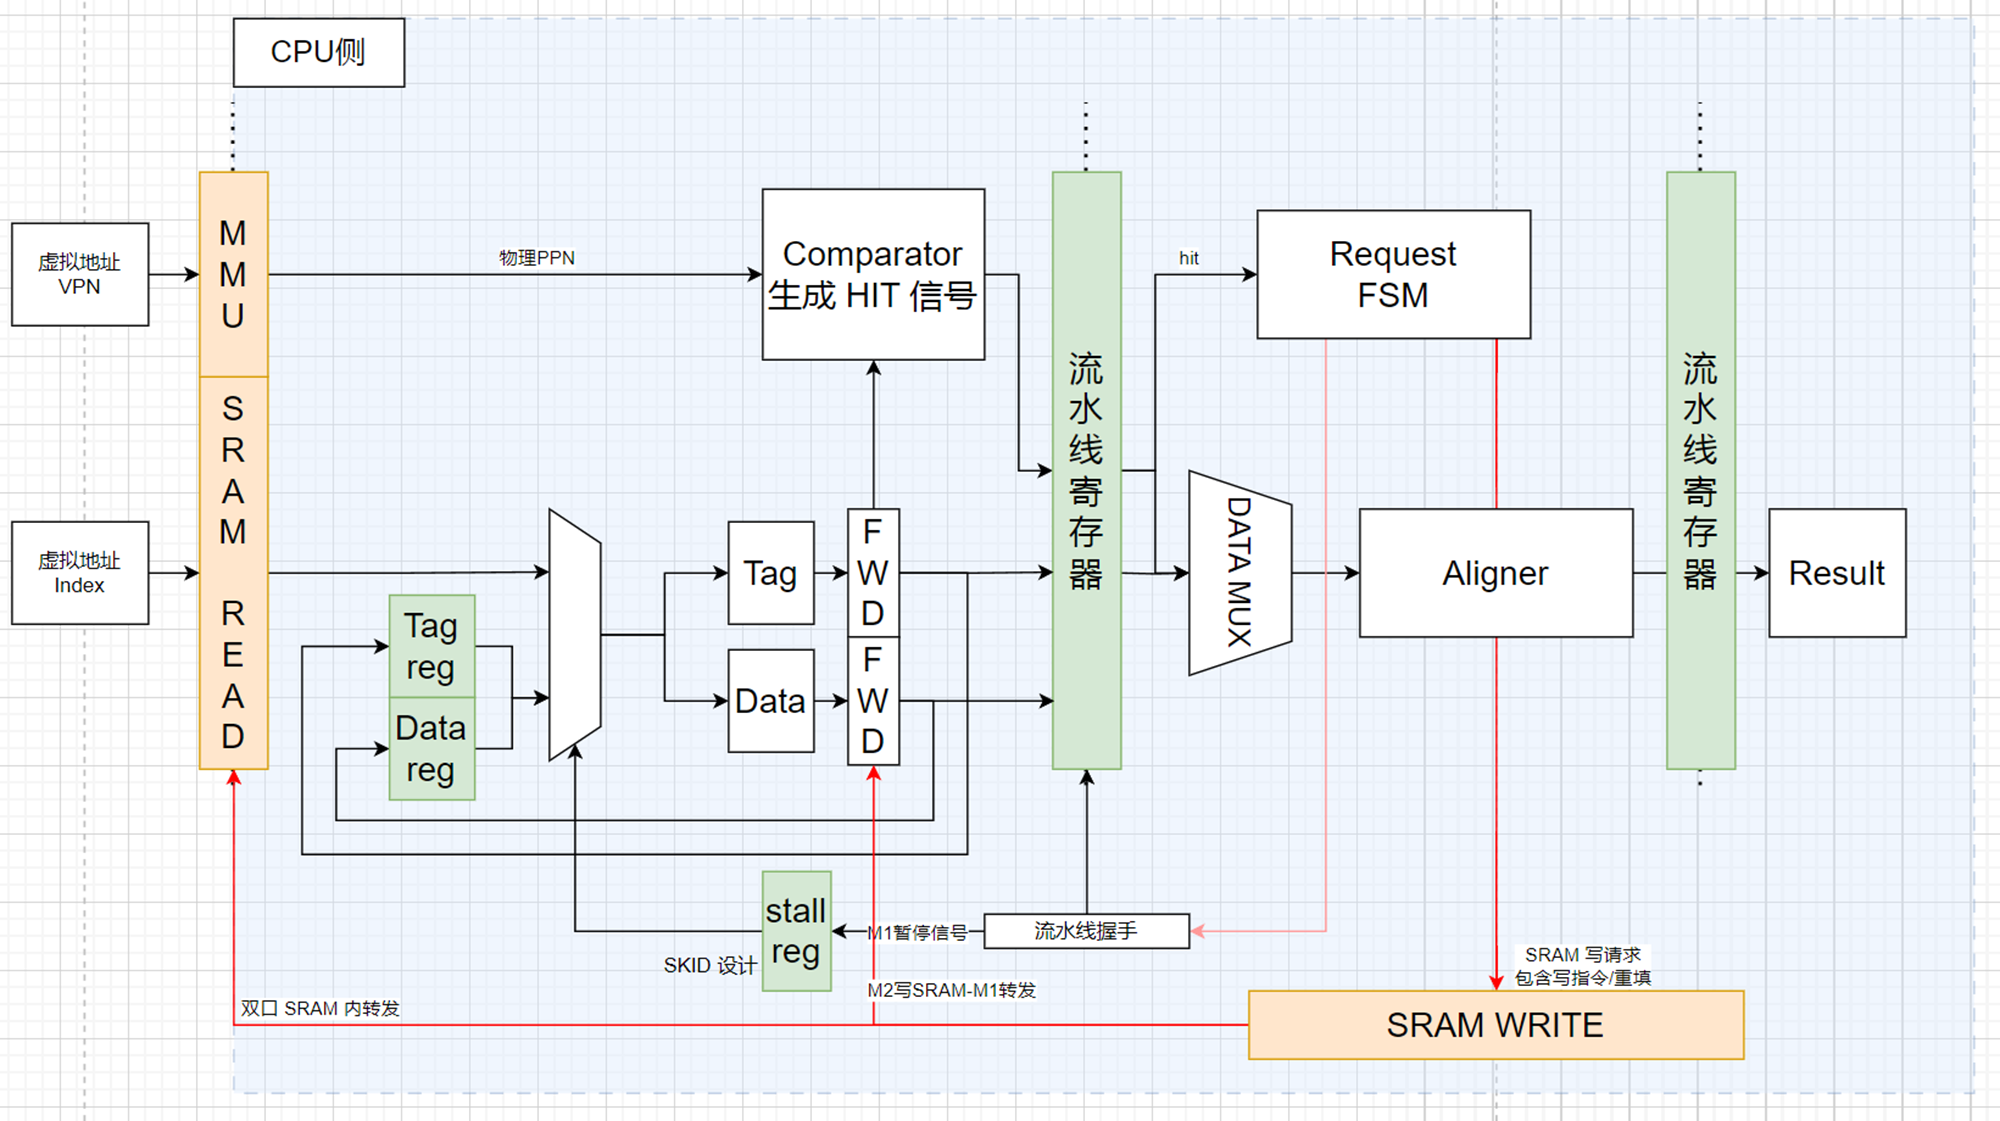
\includegraphics[width=1.0\linewidth]{assets/04/cache-arch.png}
  \caption{缓存架构图}
  \label{fig:04-cache-arch}
\end{figure}

\subsection{流水线实现细节}\label{sec:04-advanced-cpu-019}

\subsubsection{SRAM 转发}\label{sec:04-advanced-cpu-020}

LainCore 中的缓存 SRAM 读写分布在多个周期中。其中，第一个周期进行缓存 SRAM 的读取，第三个周期进行缓存 SRAM 的写入。由于 SRAM 特性，当前周期的写入在下一周期，才能被读取端口观察到，因此 LainCore 为缓存内的 SRAM 配置了两级转发。

第一级转发发生在第一级流水与第三级流水访问相同地址时。此时，直接将第三级流水写入的数据转发给第一级流水。

第二级转发发生在第二级流水与第三级流水访问相同地址时。此时，缓存丢弃第一级访问 SRAM 的结果，使用第三级写入的新数据。

\subsubsection{流水线暂停处理}\label{sec:04-advanced-cpu-021}

LainCore 内部切分了多个流水线周期，流水线暂停时也需要考虑对 SRAM 数据进行转发。Lain 中采用了一种类似 Skid Buffer 的设计处理暂停时的转发问题。

在第二级流水线中，存在一组 Skid 寄存器，暂存上一拍经过转发的最新 SRAM 数据。

同时，第二级流水线时刻追踪流水线握手信号，在流水线受到阻塞的下一拍使能一个控制信号，根据此信号控制双路选择器，使第二级流水线使用来自 Skid Buffer 的数据而不是直接来自 SRAM 的数据。 这样的实现即可保证第二级流水线始终追踪到最新的 SRAM 写入。

\subsection{流水线状态机实现}\label{sec:04-advanced-cpu-022}

\subsubsection{状态机分离设计}\label{sec:04-advanced-cpu-023}

LainCore 中的缓存状态机与缓存流水线进行了切分，两者之间采用一套请求握手机制通讯。这样做到了代码和逻辑层面的解耦，简化设计复杂度。

如下是流水线握手信号定义，流水线通过这些信号向状态机提出请求。

% 代码语言：BookSystemVerilog
\begin{CodeBlock}[language=BookSystemVerilog]
typedef struct packed {
          // 缓存请求类型
          logic cache_refill_valid;
          logic uncached_read;
          logic hit_write_req_valid;
          logic cache_op_inv;
          logic cache_op_invwb;
          logic miss_write_req_valid;
          logic uncached_write_valid;

          // 请求相关地址以及数据
          logic [31:0] addr;
          logic [1:0] rwsize;
          logic [`_DWAY_CNT - 1 : 0] wsel;
          logic [3:0] wstrobe;
          logic [31:0] wdata;

          // 写回用
          logic [`_DWAY_CNT - 1 : 0][31:0] rdata;
          dcache_tag_t [`_DWAY_CNT - 1 : 0] tag_rdata;
        } rport_state_t;
\end{CodeBlock}

在流水线状态机内部，会对这些请求进行识别与响应。核心状态机如下：

% 代码语言：BookSystemVerilog
\begin{CodeBlock}[language=BookSystemVerilog]
  // 核心状态机
  typedef logic[3:0] fsm_t;
  localparam fsm_t S_NORMAL     = 0;
  localparam fsm_t S_WB_WADR    = 1;
  localparam fsm_t S_WB_WDAT    = 2;
  localparam fsm_t S_REFIL_RADR = 3;
  localparam fsm_t S_REFIL_RDAT = 4;
  localparam fsm_t S_PT_RADR    = 5;
  localparam fsm_t S_PT_RDAT    = 6;
  localparam fsm_t S_TAG_UPDATE = 7;
  localparam fsm_t S_WAIT_BUS   = 8;
  fsm_t fsm_q, fsm;
  logic            set_ram_timer       ; // 重设 ram 计数器
  logic            set_bus_timer       ; // 重设 写回 buf 计数器
  always_ff @(posedge clk) begin
    if(!rst_n) begin
      fsm_q <= S_NORMAL;
    end
    else begin
      fsm_q <= fsm;
    end
  end
  always_comb begin
    fsm       = fsm_q;
    op_ready  = '0;
    set_ram_timer = '0;
    set_bus_timer = '0;
    case(fsm_q)
      default/*S_NORMAL*/: begin
        if(op_valid_q) begin
          case(op_type_q)
            default/*O_READ_REFILL,O_WRITE_REFILL*/: begin
              if(bus_busy_o) begin
                fsm = S_WAIT_BUS;
              end
              else begin
                if(oldtag_q.valid && dirty_rdata[refill_sel_q]) begin
                  // 脏写回
                  set_ram_timer = '1;
                  fsm       = S_WB_WADR;
                end
                else begin
                  fsm = S_REFIL_RADR;
                end
              end
            end
            O_READ_UNCACHE : begin
              if(bus_busy_o) begin
                fsm = S_WAIT_BUS;
              end
              else begin
                fsm = S_PT_RADR;
              end
            end
            O_CACHE_INV : begin
              if(bus_busy_o) begin
                fsm = S_WAIT_BUS;
              end
              else begin
                fsm = S_TAG_UPDATE;
              end
            end
            O_CACHE_INVWB : begin
              if(bus_busy_o) begin
                fsm = S_WAIT_BUS;
              end
              else begin
                if(oldtag_q.valid && dirty_rdata[refill_sel_q]) begin
                  // 脏写回
                  set_ram_timer = '1;
                  fsm       = S_WB_WADR;
                end
                else begin
                  fsm = S_TAG_UPDATE;
                end
              end
            end
          endcase
        end
      end
      S_WAIT_BUS : begin
        if(!bus_busy_o) begin
          fsm = S_NORMAL;
        end
      end
      S_WB_WADR : begin
        set_bus_timer = '1;
        if(bus_resp_i.ready) begin
          fsm = S_WB_WDAT;
        end
      end
      S_WB_WDAT : begin
        if(bus_resp_i.data_ok && bus_req_o.data_last) begin
          // todo: 明确不同类型的 op 在写回完成后的操作
          if(op_type_q == O_CACHE_INVWB) begin
            fsm = S_TAG_UPDATE;
          end
          else begin
            fsm = S_REFIL_RADR;
          end
        end
      end
      S_REFIL_RADR : begin
        set_bus_timer = '1;
        if(bus_resp_i.ready) begin
          fsm       = S_REFIL_RDAT;
        end
      end
      S_REFIL_RDAT : begin
        if(bus_resp_i.data_ok && bus_resp_i.data_last) begin
          fsm = S_TAG_UPDATE;
        end
      end
      S_PT_RADR : begin
        if(bus_resp_i.ready) begin
          fsm = S_PT_RDAT;
        end
      end
      S_PT_RDAT : begin
        if(bus_resp_i.data_ok && bus_resp_i.data_last) begin
          op_ready = '1;
          fsm = S_NORMAL;
        end
      end
      S_TAG_UPDATE : begin
        op_ready = '1;
        fsm = S_NORMAL;
      end
    endcase
  end
\end{CodeBlock}

\section{旁路结构}\label{sec:04-advanced-cpu-024}

LainCore 为顺序流水线设计，为了最大化流水线性能，需要对数据进行及早的转发前递。LainCore 处理器利用寄存器重命名的机制，对流水线前递进行了创新的优化。

数据前递是顺序核心提升 IPC 的一个重要结构设计。

对于超标量处理器，需要注意的是每个流水级目前都会存在两个转发源。

Lain Core 的转发实现逻辑与其它核心没有本质的区别，在每级流水线检查数据是否就绪以及是否本级一定需要让流水线数据就绪（若本级不就绪就放行指令会造成指令执行错误）。

若指令数据未就绪，则进行暂停检查及前递检查。

对于暂停检查，检查本级是否一定需要获取数据，若本级一定需要获取数据，则不允许指令流向下一流水级直到数据就绪。

对于前递检查，检查本级之后的所有流水级的写寄存器值和写寄存器号，追踪到最新的一条与当前读寄存器号一致的写寄存器请求进行转发前递，并保存最新的前递后的寄存器结果。

这种转发方案有一个显著的缺点，就是在每个流水级，都必须检查相应流水级之后的所有流水阶段的写寄存器情况，并进行优先级解码才能完成转发。若不监听所有流水级，则核心可能监听到错误的数据源。这样的实现会导致较长的组合逻辑链。

Lain Core 针对这个问题采用了一种比较特殊的转发设计：寄存器重命名。

Lain Core 在指令的发射检查阶段，为每个指令的所有写寄存器分配重名后的三位寄存器号，并记录寄存器号到发射重命名表（重命名分配采用类似 rob 分配的方法，使用一个计数器，每发射一对指令就增加 1）。

由于流水线长度有限，保持在流水线中而还没提交的指令总数也有限。重命名后的三位寄存器号一定不会在流水线中发生重复，也就是该寄存器号在流水线中是唯一的。

每条指令在提交，结果写回体系结构寄存器堆后，将自己重命名的寄存器号写入提交级的重命名表。

在发射阶段，只需要比较每个指令操作数对应的重命名级重命名表项值和提交级重命名表项值是否一致，即可判断体系结构寄存器堆中的值是否有效。

对于操作数还未就绪的寄存器，此时已经拿到了其重命名后的寄存器号。在管线中，一定存在唯一且确定的一个流水级的执行单元，写回的重命名寄存器号与之匹配，正存储着对应操作数的执行状态和数据。

因此，再进行数据转发时，只需要比较重命名后的寄存器号是否相等即可，相等即可转发，不再需要做优先级解码（重命名后的寄存器号唯一）。

这种实现，保证了重命名后寄存器号在管线中的唯一性，还为部分转发带来了可能。流水线级不再需要监视其后的每一级数据源，其需要监视的最小数据源仅有最后一级流水线（保证一定能拿到需要的数据）。

对于其它转发源，只需要进行可选的转发即可。

这项转发优化，将原有的转发源比较由 5位-5位 减少到 3位-3位，也规避优先级解码，整体逻辑深度在 FPGA 上有较大改善。允许部分转发，可以牺牲一点 IPC，换来较多的频率增益。
